% !TeX spellcheck = en_US
\documentclass[french]{yLectureNote}

\title{Mécanique}
\subtitle{Mécanique du point}
\author{Paulhenry Saux}
\date{\today}
\yLanguage{Français}

\professor{S.Deheuvels}%sebastien.deveuhels.irap.omp.eu

\usepackage{graphicx}%----pour mettre des images
\usepackage[utf8]{inputenc}%---encodage
\usepackage{geometry}%---pour modifier les tailles et mettre a4paper
%\usepackage{awesomebox}%---pour les boites d'exercices, de pbq et de croquis ---d\'esactiv\'e pour les TP de PC
\usepackage{tikz}%---pour deiffner + d\'ependance de chemfig
\usepackage{tkz-tab}
\usepackage{chemfig}%---pour deiffner formules chimiques
\usepackage{chemformula}%---pour les formules chimiques en \'equation : \ch{...}
\usepackage{tabularx}%---pour dimensionner automatiquement les tableaux avec variable X
\usepackage{awesomebox}%---Pour les boites info, danger et autres
\usepackage{menukeys}%---Pour deiffner les touches de Calculatrice
\usepackage{fancyhdr}%---pour les en-t\^ete personnalis\'ees
\usepackage{blindtext}%---pour les liens
\usepackage{hyperref}%---pour les liens (\`a mettre en dernier)
\usepackage{caption}%---pour la francisation de la l\'egende table vers Tableau
\usepackage{pifont}
\usepackage{array}%---pour les tableaux
\usepackage{lipsum}
\usepackage{yFlatTable}
\usepackage{multicol}
\usepackage{cancel}
\usepackage{xcolor}
\newcommand\Ccancel[2][black]{\renewcommand\CancelColor{\color{#1}}\cancel{#2}}
\newcommand{\Lim}[1]{\lim\limits_{\substack{#1}}\:}
\renewcommand{\vec}{\overrightarrow}
\newcommand{\norm}[1]{||\vec{#1}||}
\newcommand{\dd}[0]{\mathrm{d}}
\newcommand{\ddp}[0]{\partial}
%\DeclareMathOperator\arctanh{arctanh}
\DeclareMathOperator\grad{grad}
\begin{document}

%\titleOne
\setcounter{chapter}{7}
	\chapter{Puissance, travail et énergie}
\section{Puissance d'une force}
\subsection{Définition}
\begin{theorem}[Définition d'une force]
La puissance de $\vec{F}$ est donnée par
$P = \vec{F}\cdot\vec{v}$ et s'exprime en Watt ($kg\cdot m^2\cdot s^{-3}$). Elle dépend du référentiel d'étude.
\end{theorem}
\begin{multicols}{2}
La puissance est positive si $\theta \in[\frac{-\pi}{2},\frac{\pi}{2}]$. On dit que la force est motrice au temps où la puissance est calculée.\marginCritical{La puissance est instantanée. Cela signifie qu'au cours d'un mouvement, la force peut \^etre motrice ou résistante. C'est le cas de la force de rappel du ressort pendant une oscillation.}

La puissance est négative si $\theta \in[\frac{\pi}{2},\frac{3\pi}{2}]$. On dit que la force est résistante au temps où la puissance est calculée.

\columnbreak
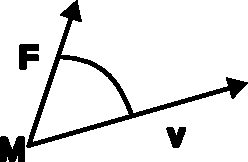
\includegraphics{path6}
\end{multicols}
\subsection{Théorème de la puissance cinétique}
\begin{theorem}[Théorème de la puissance cinétique]
La dérivée temporelle de l'énergie cinétique vaut la somme des puissances des forces exercées sur le système.
\[\dot{E_c} = \sum_i P(\vec{F_i})\]
\end{theorem}
\subsubsection{Exemple sur le pendule}
On fait un bilan des forces :
\[
 \left\{\begin{matrix}
\vec{T} =& -T\vec{e_{\rho}}\\
\vec{P} =& -mg\sin\varphi \vec{e_{\varphi}}
\end{matrix}\right.\]

$P(\vec{T}) = \vec{T}\cdot\vec{v} = (-T\vec{e_{\rho}})\cdot(l\dot{\varphi}\vec{e_{\varphi}}) = 0$ car $\vec{T}\perp \vec{v}$\marginTips{On rappelle que l'expression de la vitesse en coordonnées polaire avec un rayon constant est $\rho\dot{\varphi}\vec{e_{\varphi}}$}

$P(\vec{P}) = \vec{P}\cdot\vec{v} = -mgl\sin(\varphi)\times \dot{\varphi}$.

On applique le TPC :
\begin{flalign*}
\dot{E_c} &= P(\vec{P}) + P(\vec{T})\\
\frac{1}{2}m\frac{\mathrm{d}}{\mathrm{d}t}l^2\dot{\varphi}^2 &= -mgl\sin(\varphi)\times \dot{\varphi}\\
\frac{1}{2}\frac{\mathrm{d}}{\mathrm{d}t}l\dot{\varphi} &= -g\sin(\varphi)\\
l\ddot{\varphi} + g\sin(\varphi) &=0
\end{flalign*}

En faisant l'approximation des petits angles, on retrouve l'EQD trouvée avec l'analyse classique (PFD).\marginInfo{On perd l'information sur les forces qui sont perpendiculaires au déplacement mais on gagne en simplicité. Un raisonnement énergétique peut donc simplifier les choses.}
\section{Travail et Théorème de l'énergie cinétique}
\subsection{Travail d'une force}
Soit un système se déplaçant de A vers B suivant un chemin $C(AB)$. On veut connaitre le travail d'une force $\vec{F}$ lors de ce déplacement. On décompose le chemin en déplacements élémentaires $\mathrm{d}\vec{r}$ et on introduit le travail élémentaire $\delta W$\marginInfo{On l'écrit $\delta W$ et non $\mathrm{d} W$, car généralement, ce n'est pas la différentielle d'une fonction $W$ car cela signifirait que $\in_A^B\mathrm{d}f = f(B)-F(A)$ et donc que $W$ ne dépend que des points et non du chemin.}, avec $\delta W = \vec{F} \cdot \mathrm{d}\vec{r}$\marginTips{En effet, $\vec{F}$ est considérée comme constante sur ce petit déplacement.}

On a alors le travail de la force F sur le chemin $C(AB)$\marginInfo{Aussi appelé circulation du vecteur $\vec{F}$ sur le chemin $C(AB)$}
\begin{equation}
 W_{C(AB)} (\vec{F}) = \int_{C(AB)}\delta W = \int_{C(AB)} \vec{F} \cdot \mathrm{d}\vec{r}
\end{equation}
\subsubsection{Propriétés}
\begin{itemize}
 \item On peut séparer le chemin en morceau, puis sommer les travaux
 \item Si on parcourt le chemin dans l'autre sens, le travail sera opposé.
 \item Généralement, la circulation dépend du chemin emprunté entre les 2 points.
 \item Si $W > 0$, la force est dite motrice, dans le cas contraire elle est négative, si $W=0$, la force ne travaille pas.
\end{itemize}
\subsubsection{Déplacement élémentaire}
On a $\vec{v} = \frac{\mathrm{d}\vec{r}}{\mathrm{d}t} \iff \mathrm{d}\vec{r} = \vec{v}\times \mathrm{d}t$.

En cartésien à 3D : $\mathrm{d}\vec{r} = \mathrm{d}x\vec{e_x} + \mathrm{d}y\vec{e_y} + \mathrm{d}z\vec{e_z}$

En cylindrique : $\mathrm{d}\rho\vec{e_{\rho}} + \rho\mathrm{d}\varphi\vec{e_{\varphi}} + \mathrm{d}z\vec{e_z}$.
\subsection{Calcul du travail d'une force}
\subsubsection{Forces $\perp$ au mouvement}
Elles ne fournissent aucun travail.
\subsubsection{Cas d'une force constante}
On a $W_{C(AB)} (\vec{F}) = \int_{C(AB)} \mathrm{d}\vec{r} = \vec{F} \cdot\int_{C(AB)} \mathrm{d}\vec{r} = \vec{F} \cdot \vec{AB}$.\marginCritical{En effet, la somme de tous les \emph{vecteurs} petits déplacement élémentaires donne $\vec{AB}$. Ce n'est pas la somme de la quantité scalaire mais bien la somme des vecteurs car la somme des quantités $\dd t$ donne la longueur du chemin parcourue !}
\subsubsection{Forces non constantes}
Voir fiche de méthodologie pour plus d'exemples.
\subsection{Théorème de l'énergie cinétique}
\begin{theorem}[Énoncé]
\[\Delta_{AB} E_c = \sum_i W_{C,AB}(\vec{F_i})\]
\end{theorem}
\section{Énergie potentielle et forces conservatives}
\subsection{Notion de forces conservatives}
% \subsubsection{Notion de différentielle}
% Pour une fonction $f$ qui est $C^1$, on peut définir $\dd f(a) = f(a+\dd x) - f(a)$.
%
% La dérivée est $f'(a) = \Lim{\dd\to 0} \frac{f(a+\dd x)-f(a)}{\dd x}$.
%
% On a donc $\dd f(a) = f'(a)\dd x \iff f'(a) = \frac{\dd f(a)}{\dd x}$. On peut le généraliser au cas de fonctions de plusieurs variables $f(x,y,z)$ et obtenir des dérivées partielles pour chaque variables.
%
% $\dd f = \frac{\partial f}{\partial x}\dd x + \frac{\partial f}{\partial y}\dd y + \frac{\partial f}{\partial z}\dd z$.
\subsubsection{Force conservative}
\begin{definition}[Définition 1]
Une force $\vec{F}$ est dite conservative s'il existe une fonction $u(\vec{r})$ de l'espace tel que le travail élémentaire $\delta W(\vec{F}) = \vec{F}\cdot \dd \vec{r}$ soit égal à $\delta W = -\dd u$.
\end{definition}
\begin{definition}[Définition 2]
Une force est conservative $\iff$ le travail de $\vec{F}$ dans le déplacement de A vers B ne dépend pas du chemin pris.
\end{definition}
\begin{definition}[Définition 3]
$\vec{F}$ est conservative $\iff$ le travail sur tout chemin fermé est nul (le point de départ = point d'arrivée).
\end{definition}
\subsection{Énergie potentielle}
\begin{definition}[Énergie potentielle]
Si une force $\vec{F}$ est conservative, il existe une fonction $u$ telle que $\delta W(\vec{F}) = -\dd u$. On appelle $u$ énergie potentielle, notée $E_{P_F}$.
\end{definition}

Ainsi, $W(\vec{F}) = \int \delta W = -\int dE_p = -E_p(B)-E_p(A)$. La variation d'énergie potentielle sur $AB$ vaut l'opposé du travail\marginCritical{Le travail étant le résultat d'une intégrale, l'énergie potentielle est définit à une constante près. Il faut donc se fixer un point de référence où elle est nulle.}, autrement dit\marginTips{On peut dire aussi $\Delta E_p$ vaut le travail qu'un utilisateur doit fournit pour amener le système du point A au point B.} :\[\Delta_{AB} E_p = -W_{C,AB}(\vec{F})\]
\subsubsection{Méthode}
Voir fiche de méthodologie
\subsection{Opérateur gradient}
Le vecteur gradient en cartésien  est :\marginInfo{L'expression du gradient dépend du système de coordonnées dans lequel on se trouve}
\[\grad(u) =  \begin{pmatrix}
\frac{\partial u}{\partial x} \\
 \frac{\partial u}{\partial y}\\
 \frac{\partial u}{\partial z}
\end{pmatrix}\]

\subsubsection{Propriétés}
\begin{itemize}
 \item Il est linéaire
 \item Il est dirigé dans le sens des $u$ croissants, c'est à dire pour maximiser l'augmentation de $u$.
 \item Il est orthogonal aux équipotentielles de $u$, surfaces sur lesquelles $u$ est constant.
\end{itemize}
\subsection{Calcul de $E_p$ avec le gradient}
\begin{definition}[Définition 4 d'une force conservative]
Une force $\vec{F}$ est conservative $\iff$ il existe une fonction $E_p$ telle que $\vec{F} = -\grad(E_p)$. On dit que $\vec{F}$ dérive d'une énergie potentielle.
\end{definition}
\subsection{Calcul de $E_p$ pour des forces conservative}
	\begin{tabular}{_l^l^l}
		\tableHeaderStyle%
		Force & Expression & Énergie potentielle\\
		Force de rappel & $\vec{F_r} = -kx\vec{e_x}$ & $\frac{kx^2}{2}$\\
		Force de gravitation & $\vec{F_g} = -\frac{GMm}{r^2}\vec{e_r}$ & $E_p = -GmM\frac{1}{r}$\\
		Force électrostatique & $\vec{F_e} = -\frac{qq_0}{4\pi\varepsilon_0\times r^2}$ & $E_p = -\frac{1}{4\pi\varepsilon_0}\times\frac{qq_0}{r}$\\
	\end{tabular}

Ces expressions peuvent \^etre différentes selon les axes et bases utilisés.
\section{Énergie mécanique}
\subsection{Théorème de l'énergie mécanique}
\begin{theorem}[]
La variation de l'énergie mécanique correspond à la somme des travaux des forces non conservatives, qui dissipent de l'énergie, comme les frottements. \[\Delta_{AB}E_m = \Delta_{AB}E_c + \sum_i \Delta_{AB}E_{p,i} = \sum_i W_{C,AB}(\vec{F_{NC}})\]
\end{theorem}
Sans forces non conservatives, l'énergie mécanique se conserve.\marginTips{Si les forces conservatives en présence ont des $E_p$ connues, on utilise plut\^ot ce théorème.}
\subsection{Théorème de la puissance mécanique}
\begin{theorem}[TPM]
\[\frac{\dd E_m}{\dd t} =\sum_j P(\vec{F_{NC,j}})\]
\end{theorem}

\section{Interprétation graphique de l'énergie potentielle}
On s'intéresse à des systèmes dont le mouvement possède un seul degré de liberté.\marginTips{Un seul paramètre décrit le mouvement (cas d'un mouvement rectiligne par exemple, mouvement circulaire à rayon constant)} et conservatif. On considère $E_p$ la somme de toutes les énergies potentielles. On note $\vec{F}$ la résultante des forces. $E_p$ correspond donc à l'énergie potentielle associée à $\vec{F}$.

Il y a un seul degré de liberté : $\vec{F}(x) = F(x)\vec{e_x}$. On peut écrire $\vec{F} = -\grad(E_p)\Rightarrow F(x) = -\frac{\dd E_p}{\dd x}$.

On peut alors interpréter le graphique $E_p$ en fonction de $x$.

\subsubsection{Position d'équilibre}
L'accélération est nulle, donc $\vec{F} = \vec{0} \iff -\frac{\dd E_p}{\dd x} =0$, donc les positions d'équilibre correspondent aux points où la courbe $E_p(x)$ admet une tangente horizontale.\marginTips{Cela peut se produire aux extremum locaux, mais aussi aux points d'inflexion.}
\subsubsection{Signe de la dérivée}
Si $\frac{\dd E_p}{\dd x}>0, F(x)<0$ ($E_p$ croissante)

Si $\frac{\dd E_p}{\dd x}<0, F(x)>0$

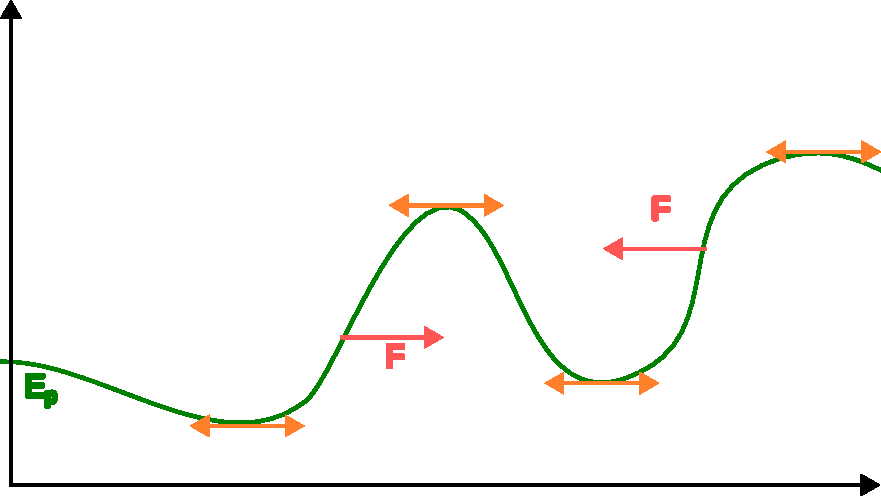
\includegraphics[scale=0.5]{graph}
\subsection{Stabilité des positions d'équilibre}
\begin{definition}
Une position d'équilibre est stable si les forces en présence tendent le système à s'y ramener.
\end{definition}
\subsubsection{Condition pour qu'une position d'quilibre soit table}
Soit $x_0$ une positon d'équilibre, $F(x) = 0 \iff -\frac{\dd E_p}{\dd x} = 0$\marginCritical{Il s'agit bien de la dérivée en fonction de $x$ en non la dérivée temporelle}

Pour qu'une position soit stable, il faut que $F(x_0+\dd x)<0$ quand $x>0$ ou $F(x_0+\dd x)>0$ quand $x<0$

On réécrit la première égalité :
\begin{flalign*}
 \frac{F(x_0+\dd x)-F(x_0)}{\dd x} &< 0\\
 \frac{\dd F}{\dd x}(x_0) &< 0 \iff -\frac{\dd^2 E_p}{\dd x^2} <0\\
 \frac{\dd^2 E_p}{\dd x^2}&>0
\end{flalign*}
Il faut donc que la courbe soit convexe en $x_0$

En ajoutant l'information de l'$E_m$, on peut conna\^itre l'évolution du système. On peut se représenter des puits\marginInfo{Un puits d'énergie potentielle existe lorsque la représentation graphique de l'énergie potentielle en fonction du paramètre décrivant le mouvement admet un puits. Si le système n'a pas assez d'énergie mécanique pour sortir du puits, il est contraint de rester entre deux positions et peut éventuellement osciller.} et barrières de potentiel\marginInfo{Une barrière d'énergie potentielle existe lorsque  le système ne peut alors pas aller au-delà de cette position, faute d'énergie suffisante et est contraint de revenir en arrière.}

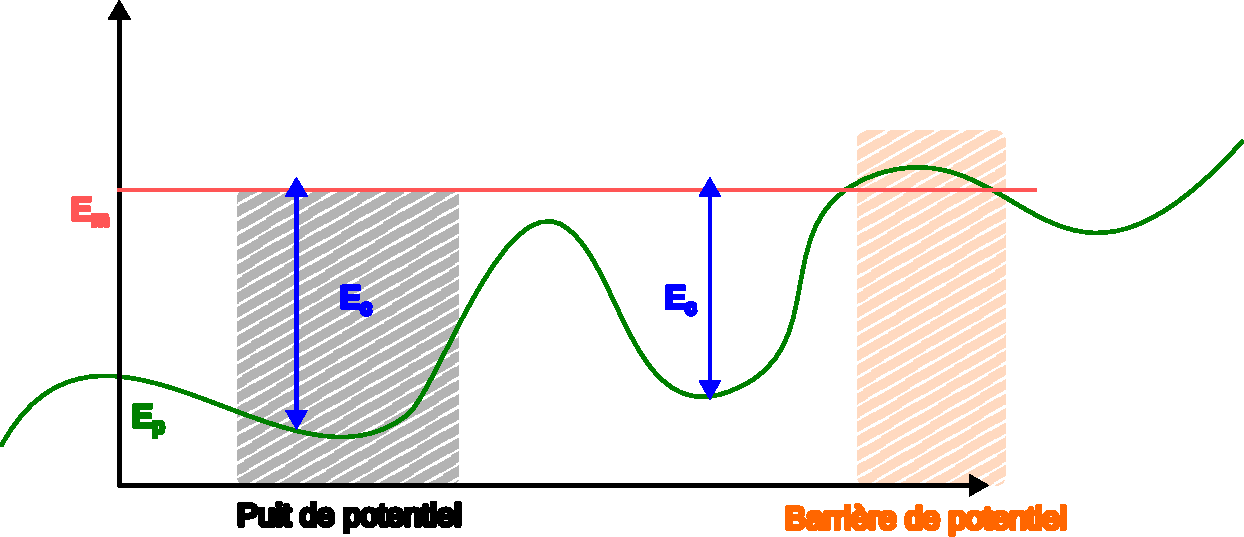
\includegraphics[scale=0.5]{rect5}

\end{document}
